% LTeX: language=pt-BR

\section{Estado da Arte}\label{sec:art}

A comunidade científica e de analistas trabalham ativamente em diversas frentes contra vulnerabilidades. Discutimos a cinco estágios do processo de mitigação de vulnerabilidades de \emph{software}: identificação de vulnerabilidades via análise de código (Seção~\ref{sec:art.ident}), detecção de vulnerabilidades em produção (Seção~\ref{sec:art.detect}), catalogação de vulnerabilidades (Seção~\ref{sec:art.data}), modelagem de vulnerabilidades (Seção~\ref{sec:art.model}) e priorização de vulnerabilidades (Seção~\ref{sec:art.prio}). Damos foco especial nas bases de dados que catalogam diversas informações sobre vulnerabilidades e mecanismos de priorização (Seções~\ref{sec:art.data} e~\ref{sec:art.prio}).

% \begin{figure}
%   \centering
%   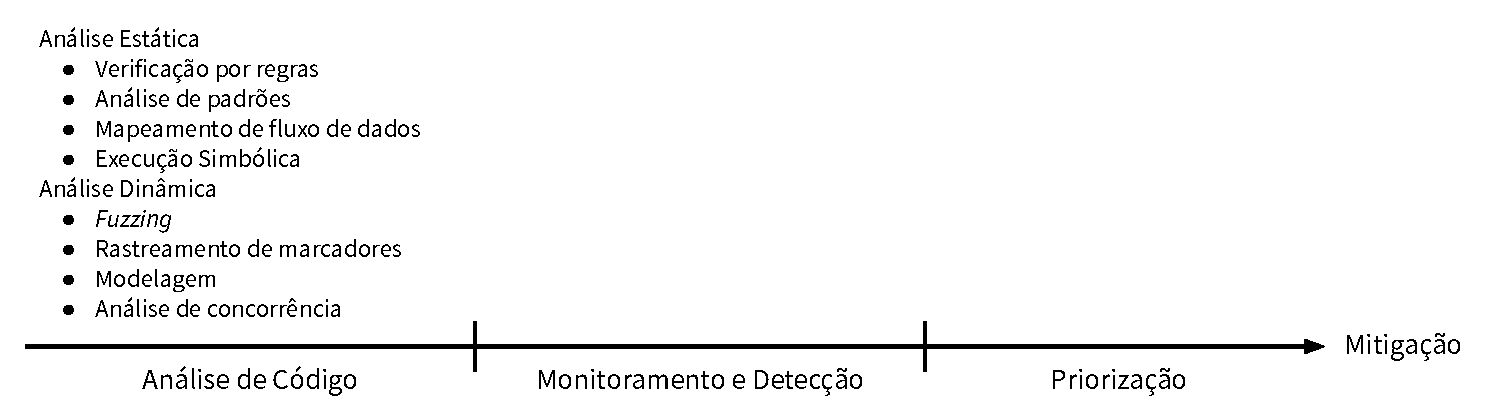
\includegraphics[width=\textwidth]{figs/GT-Crivo-Bibliography-Review-Overview.pdf}
%   \caption{Estágios no processo de mitigação de vulnerabilidades de \emph{software}.}\label{fig:art.stages}
% \end{figure}

\subsection{Identificação de Vulnerabilidades via Análise de Código}\label{sec:art.ident}

A identificação de vulnerabilidades a partir da análise do código de um programa permite mitigação antes do programa ser distribuído e entrar em operação, contribuindo significativamente para a melhoria da qualidade do \emph{software} e segurança de sistemas~\cite{lin20vuln, zeng20vuln, semasaba20survey}.

A análise estática de código verifica propriedades de um programa a partir de seu código-fonte, sem executá-lo. Abordagens comuns para análise estática de código incluem:

\begin{description}

  \item[Verificação por regras~\cite{engler01bugs, chen2017efficient}.] A verificação por regras garante que o código segue um conjunto pré-definido de regras. Regras podem especificar requisitos de segurança como restringir algoritmos criptográficos a versões seguras, verificar a configuração de algoritmos criptográficos e exigir que entradas de usuário ou recebidas pela rede sejam validadas antes de serem usadas. A verificação por regras aborda aspectos específicos do código de forma determinística.

  \item[Análise de padrões~\cite{jang12redebug, kim17vuddy}.] A análise de padrões envolve análise de código para identificar padrões e verificar propriedades gerais. Por exemplo, a análise de padrões pode verificar a aderência a melhores práticas e convenções, bem como a utilização de padrões de projeto (\emph{design patterns}) adequados. A análise de padrões toma uma visão mais ampla do código, com resultados potencialmente ambíguos ou incompletos.

  \item[Mapeamento de fluxo de dados~\cite{qin06lift, chang08dataflow}.] O mapeamento de fluxo de dados envolve identificar as fontes dos dados utilizadas pelo programa e construir um grafo do fluxo dos dados através das manipulações, operações e transformações realizadas pelo programa. O grafo permite inferir propriedades sobre as saídas geradas pelo programa, por exemplo, se existe possibilidade de vazamento de dados sensíveis em alguma saída. A análise de fluxo de dados também permite identificar vulnerabilidades como uso de variáveis não inicializadas. Por último, o mapeamento do fluxo de dados permite identificar quais variáveis dependem de dados recebidos do usuário ou da rede e podem exigir validação.

  \item[Execução simbólica~\cite{ramos15symbolic, cadar08klee, avgerinos14exploit}.] A execução simbólica de código permite inferir propriedades sobre qual código (fluxo de execução) de um programa é executado para cada entradas. A execução simbólica faz esse mapeamento para todos os possíveis fluxos de execução para todas as possíveis entradas, provendo um panorama completo do comportamento de um programa. A execução simbólica permite identificar discrepâncias semânticas entre entradas e o código executado, geralmente devido à presença de erros ou violação de alguma suposição embutida no código.

\end{description}

A análise dinâmica de código verifica propriedades de um programa durante sua execução. A análise dinâmica depende da instrumentação do código, que pode ser provida por um interpretador, máquina virtual, ambiente de execução (\emph{runtime}) ou um compilador. Algumas abordagens para análise dinâmica de código incluem:

\begin{description}

  \item[Testes com \emph{fuzzing}~\cite{pewny14signatures, sutton2007fuzzing, takanen2018fuzzing}.] Estas técnicas visam testar a execução de um programa com um grande conjunto de entradas. Entradas podem ser geradas aleatoriamente por \emph{fuzzers} caixa-preta~\cite{takanen2018fuzzing} ou geradas de forma sistemática por \emph{fuzzers} caixa-branca, que visam minimizar o número de entradas sem sacrificar ou até aumentando a cobertura do código testado.
  \emph{Fuzzers} caixa-branca podem utilizar outras técnicas de análise de código no processo de geração de entradas, como rastreamento de marcadores~\cite{ganesh2009fuzzing}, modelagem~\cite{pham2016fuzzing}, ou execução simbólica~\cite{godefroid2008fuzzing}.

  \item[Rastreamento de marcadores (\emph{taint tracking})~\cite{newsome2005dynamic, portokalidis06argos, tian2023podft, she2020neutaint}.]  Similar ao mapeamento de fluxo de dados realizado em análise estática, o rastreamento de marcadores utiliza instrumentação de código para rastrear dependências de dados durante a execução de um programa. A análise dinâmica permite melhor cobertura do código de um programa, particularmente de aspectos dinâmicos que não podem ser exercitados estaticamente, e reduz a quantidade de falsos positivos ao reportar sobre observações diretas da execução do código, por exemplo, ao observar vazamentos concretos de dados sensíveis.

  \item[Modelagem.] A execução dinâmica de código e verificação de propriedades pode tomar várias formas, dependendo principalmente de propriedades conhecidas de um programa que podem ser capturadas por modelos. Por exemplo, a verificação de invariantes~\cite{lin2021inferring, lin2021inferring} permite verificar se propriedades predeterminadas conhecidas que deveriam ser mantidas por um programa (\emph{e.g.,} em um laço) são realmente mantidas durante toda a execução de um programa.  De forma geral, modelos podem ser utilizados para verificar propriedades de um programa analisado estaticamente ou executado dinamicamente, por exemplo, através de arcabouços para interpretação abstrata de programas~\cite{stein2021demanded, vedrine2021runtime}.  A violação de um modelo durante a execução dinâmica de um programa permite a identificação de erros, melhorando corretude e reduzindo vulnerabilidades.

  \item[Detecção de erros de concorrência~\cite{silva2020shake, cai2021sound}.] Erros de concorrência como condições de corrida e \emph{deadlocks} em programas paralelos ou sistemas distribuídos são sérias fontes de erros e vulnerabilidades. Sua detecção é complicada pela dificuldade de reproduzir estes erros. Uma abordagem para identificar erros de concorrência é intercalar de forma sistemática o escalonamento de \emph{threads} de um programa~\cite{chen2020muzz, gong2021snowboard}. Outra abordagem é instrumentar código para rastrear a ordem de acessos à memória e a recursos com o objetivo de identificar sequências inválidas de acesso como uso de dados desatualizados ou não inicializados.

\end{description}

Resultados de pesquisa são frequentemente integrados ou disponibilizados como ferramentas. A comunidade científica e de analistas de segurança desenvolve e mantêm dezenas de ferramentas para análise estática e dinâmica de código~\cite{beller16static, gosain15dynamic}. Ferramentas de análise de código têm ganhado popularidade e seu uso vem aumentando concomitante à adoção de arcabouços de integração contínua (CI) por diversos projetos de \emph{software}~\cite{sadowski2018lessons, zampetti2017open}. Apesar dos avanços na análise estática e dinâmica de código, dois desafios limitam sua acurácia e cobertura: (i) a dificuldade de inferir, na análise estática, e exercitar, na análise dinâmica, todos os estados e sequências de eventos possíveis na execução de um programa~\cite{chen2020muzz}; e (ii) o alto custo computacional de técnicas avançadas~\cite{stein2021demanded}.
A quantidade crescente de vulnerabilidades descobertas após a distribuição de \emph{software} indica que as técnicas e ferramentas atuais têm cobertura limitada face à complexidade de sistemas modernos~\cite{votipka18vuln, li18vuldeepecker}, justificando a implantação de sistemas complementares para detecção de vulnerabilidades que discutimos a seguir.

\subsection{Detecção de Vulnerabilidades via Monitoramento}\label{sec:art.detect}

A comunidade científica e de analistas de segurança trabalha continuamente no desenvolvimento de novas ferramentas para monitoramento e descoberta de vulnerabilidades de segurança~\cite{bau10scanning, doupe2010johnny, figueroa2020survey, roy2022survey}. Este esforço é essencial para entender como detectar vulnerabilidades em programas e sistemas em uso, ponto de partida para esforços de mitigação e suporte a operação continuada destes sistemas. De forma complementar, a pesquisa em métodos de monitoramento e deteção permite antecipar e desenvolver contramedidas contra ataques perpetrados por agentes maliciosos.

O monitoramento e levantamento de informações para fins de exploração de vulnerabilidades pode considerar diversos alvos~\cite{roy2022survey}: indivíduos, perfis e contas de usuários em um sistema, organizações, informações sobre infraestrutura física como configurações de \emph{hardware} e topologia de rede, bem como programas e serviços executando em um dispositivo. Apesar de estarem fora do escopo deste relatório, é importante ressaltar que a combinação de diversas fontes de informação é utilizada para realizar sofisticados ataques~\cite{hassan2018technical, albladi2018user}; exemplos incluem o ataque cibernético contra a malha elétrica da Ucrânia~\cite{defense16ukraine} e o cibergolpe contra o Banco de Bangladesh~\cite{hill18heist}.

No restante desta seção focamos no monitoramento e descobrimento de vulnerabilidades de \emph{software} que podem ser exploradas remotamente através de uma rede, uma classe de vulnerabilidades de alto risco devido à facilidade de serem exploradas. Agrupamos as diversas técnicas existentes para levantar informações e identificar vulnerabilidades em dispositivos em duas classes:

\begin{description}

  \item[Varredura de rede (\emph{scanning})~\cite{bhuyan2011surveying, barnett2008towards, wen2015novel, de1999review}.] A varredura de rede é uma técnica para identificar dispositivos ativos em uma rede e aplicações acessíveis pela rede. Varreduras de rede podem utilizar ou combinar pacotes ICMP, TCP e UDP com diferentes propriedades (e.g., portas e \emph{flags} TCP) para induzir uma resposta de dispositivos ativos~\cite{abu2006multifaceted,durumeric2013zmap}. Técnicas de varredura também podem estabelecer conexões e comunicar com uma aplicação, através de protocolos específicos utilizados pela aplicação, para obter informações adicionais~\cite{bajpai2018art,durumeric2015search}. Por exemplo, este tipo de varredura frequentemente visa obter \emph{banners}, uma resposta de um serviço que frequentemente permite identificar a aplicação e a versão escutando em uma porta de rede. \emph{Malwares} implementam diversos mecanismos de varredura de rede para maximizar a quantidade de dispositivos vulneráveis identificados~\cite{abu2006multifaceted, antonakakis17mirai, marzano18botnets}.

  \item[\emph{Fingerprinting}~\cite{bifulco2015fingerprinting, owens11fingerprint, shaikh2008network, shamsi2015hershel, shamsi2021faulds}.]  Esta técnica permite identificar propriedades de um dispositivo ou aplicação, como modelo, sistema operacional, ou versão de um \emph{software} (mesmo quando uma aplicação não envia um \emph{banner}). Isto é feito através de observações do comportamento do dispositivo ou aplicação alvo em cenários específicos. As observações podem ser coletadas por sondagem ativa ou através da observação passiva de tráfego de rede por longos períodos.
  Estas observações permitem construir uma assinatura do tráfego de uma aplicação ou dispositivos, permitindo compará-lo com um conjunto de assinaturas conhecidas. Por exemplo, o sistema operacional de um dispositivo pode ser inferido observando como ele inicializa o campo ID de pacotes IP~\cite{kohno2005remote}, como trata pacotes com a opção de \emph{Record Route}~\cite{sherwood08discarte}, ou qual algoritmo de controle de congestionamento ele utiliza no protocolo TCP~\cite{beverly2004robust}.

  % Website fingerprinting \cite{mansfield2009simple, panchenko2016website, hayes2016k}: Not really related to scanning, these are about identifying which website a user is accessing based on traffic patterns (even if the website is encrypted).

\end{description}

A seguir discutimos quatro dimensões que perpassam o projeto e execução de soluções de monitoramento de rede para detecção de vulnerabilidades:

\begin{description}

  \item[Eficiência e escalabilidade.] Uma barreira ao monitoramento de vulnerabilidades de rede é o tamanho da Internet. Monitorar bilhões de dispositivos conectados à Internet requer quantidade significativa de recursos de rede; primariamente banda de rede, mas a quantidade de pacotes frequentemente pode colocar carga significativa em roteadores~\cite{beverly10hifreq, cunha14dtrack}. Para agravar esta situação, a dinamicidade dos dispositivos implica a necessidade de monitoramento constante para manter uma visão atualizada do estado da rede. Diversos esforços na literatura visam reduzir o número de sondas necessárias para monitoramento de rede~\cite{beverly10hifreq, luckie13speedtrap, xia2005efficient, you2019profuzzer} e a velocidade com a qual a sondagem pode ser realizada~\cite{durumeric2013zmap, durumeric2015search}.

  \item[Furtividade.] Algumas técnicas de sondagem e \emph{malware} utilizam mecanismos sofisticados para realizar varreduras de rede, coletando informações por longos períodos sem serem detectados~\cite{staniford2002practical, stojanovic2020apt}.  Por exemplo, estas técnicas podem minimizar o número de pacotes enviados, distribuir o processo de sondagem no tempo e no espaço (entre diversos dispositivos alvo), falsificar o endereço IP de origem (\emph{spoofing}) para mascarar a fonte do ataque, ou utilizar técnicas de sondagem modificadas para contornar dispositivos de monitoramento~\cite{dainotti2012analysis}.

  \item[Seleção de alvos.] A seleção de alvos para uma varredura de rede envolve diversas decisões. Uma varredura pode ser vertical, focando em múltiplas portas de rede de um único dispositivo para identificar todas as aplicações em execução, ou horizontal, focando em uma porta de vários dispositivos para identificar dispositivos executando uma aplicação específica~\cite{barnett2008towards}. Para varreduras horizontais, os endereços IPs podem ser obtidos de uma lista pré-construída (\emph{hitlist}) ou a partir de prefixos IP (e.g., controlados por uma rede ou instituição alvo), os endereços podem ser sondados de forma exaustiva ou seletiva, e a ordem de sondagem pode ser sequencial, aleatória, ou seguindo alguma priorização específica~\cite{achleitner2016cyber}. Para varreduras verticais, todas as portas podem ser sondadas, ou um subconjunto de portas alvo pode ser considerado~\cite{abu2006multifaceted}. Varreduras híbridas combinam propriedades de varreduras verticais e horizontais, cobrindo múltiplas portas de diversos dispositivos.

  \item[Abordagem de medição.] A varredura de rede pode ser realizada de forma passiva, observando o tráfego de rede, ou de forma ativa, enviando pacotes de sondagem para dispositivos na rede~\cite{beverly10hifreq, luckie13speedtrap, xia2005efficient, you2019profuzzer}. Abordagens ativas incorrem custo adicional de medição, mas permitem escolha dos alvos e das técnicas de sondagem. Abordagens passivas não incorrem custo adicional de medição, são mais difíceis de detectar, mas são aplicáveis apenas aos dispositivos e aplicações enviando tráfego através da rede monitorada~\cite{yao10traceback, yao15traceback, hiesgen2022spoki}.

\end{description}

\subsection{Bases de Dados Públicas}\label{sec:art.data}

Nesta seção discutimos as diversas bases de dados sobre vulnerabilidades de \emph{software} disponíveis para analistas de segurança. Na medida do possível agregamos diversas bases de dados por tipo ou similaridade.

\begin{description}

  \item[Catalogação de vulnerabilidades.] A catalogação de vulnerabilidades é um esforço coordenado contínuo para coletar, verificar e manter informações sobre vulnerabilidades de \emph{software}. O CVE (\emph{Common Vulnerabilities and Exposures})~\cite{mell2002cve} é o mais amplo destes esforços, catalogando vulnerabilidades reportadas por desenvolvedores, analistas, pesquisadores e fabricantes. O CVE permite identificar vulnerabilidades de forma única, facilitando a gerência de vulnerabilidades. O CVE é o conjunto de dados mais frequentemente utilizado em pesquisas sobre vulnerabilidades~\cite{le2021survey}. Outras bases de vulnerabilidades existem, como o NVD (\emph{National Vulnerability Database}), mantido pelo NIST (\emph{National Institute of Standards and Technology}), o descontinuado OSVDB (\emph{Open Source Vulnerability Database}), bem como as bases da Snyk e VulDB.\footnote{\url{https://nvd.nist.gov}, \url{https://security.snyk.io} e \url{https://vuldb.com}}

  O CVD (\emph{Coordinated Vulnerability Disclosure})\footnote{https://www.cisa.gov/coordinated-vulnerability-disclosure-process} descreve o processo de divulgação de vulnerabilidades e visa garantir que vulnerabilidades sejam divulgadas de forma responsável, minimizando o risco de exploração por agentes maliciosos. As etapas do processo incluem a coleta e análise de dados sobre vulnerabilidade, notificação de desenvolvedores e fabricantes responsáveis, implementação e aplicação de medidas corretivas, bem como a divulgação simultânea por fabricantes, prestadores de serviço, distribuidores de \emph{software} e pelo CVE\@.

  \item[Ranqueamento de vulnerabilidades.] Diversas bases de dados ranqueiam vulnerabilidades de acordo com critérios específicos. Por exemplo, o CVSS (\emph{Common Vulnerability Scoring System})~\cite{mell2006cvss} é um sistema de ranqueamento de vulnerabilidades que visa padronizar a avaliação de vulnerabilidades em função de propriedades como vetor de ataque, complexidade de exploração e a necessidade de interação de um usuário. O EPSS (\emph{Exploit Prediction Scoring System})~\cite{jacobs2021epss} é um sistema de ranqueamento de vulnerabilidades que visa prever a probabilidade de uma vulnerabilidade ser explorada em um futuro próximo utilizando dados complementares, por exemplo, monitoramento de discussão de uma vulnerabilidade em redes sociais como Twitter. O catálogo KEV (\emph{Known Exploited Vulnerabilities}) é uma lista de vulnerabilidades para as quais há comprovação de exploração em ataques reais~\cite{lim23kve}.

  \item[Metadados sobre vulnerabilidades.] O CVE está fortemente acoplado a outras bases de dados que complementam informações sobre vulnerabilidades. Em particular, o \emph{Common Weakness Enumeration} (CWE)~\cite{martin2008cwe} identifica a causa raiz de uma vulnerabilidade, como validação incorreta de entrada ou escrita fora dos limites de um \emph{buffer}. O CWE tem aplicação no projeto de mitigações e contramedidas para vulnerabilidades e auxilia no direcionamento de esforços de desenvolvimento para prevenir a introdução de causas comuns de vulnerabilidades. CVEs também são frequentemente relacionados a CPEs (\emph{Common Platform Enumeration})~\cite{cheikes2011cpe}, que identificam produtos e versões de \emph{software} afetadas por uma vulnerabilidade. O CPE é útil para analistas de segurança que precisam identificar quais sistemas são afetados por uma vulnerabilidade.

  \item[Provas de conceitos e \emph{exploits}.] Bases de dados de \emph{exploits} são repositórios de códigos que exercitam e demonstram a exploração de uma vulnerabilidade. Estas bases de dados são frequentemente utilizadas para comprovar a existência da vulnerabilidade, detectar sua presença em sistemas em operação e para avaliar a eficácia de contramedidas. Exemplos de bases de dados de \emph{exploits} incluem Exploit-DB, 0day.today, Packet Storm e Metasploit.\footnote{\url{https://www.exploit-db.com}, \url{https://0day.today}, \url{https://packetstormsecurity.com} e \url{https://www.metasploit.com}} Uma limitação destas bases de dados é que elas disponibilizam provas de conceito, mas \emph{exploits} utilizados para realizar ataques reais são muito mais complexos e raramente obtidos para estudo pela comunidade de segurança~\cite{jacobs20exploit,sabottke2015vulnerability}.

  \item[Informações de rede.] Diversas informações de rede são públicas e podem prover informações complementares relacionadas a vulnerabilidades. Por exemplo, registros de numeração coletam e disponibilizam informações sobre detentores de prefixos IP e nomes de domínio através dos protocolos WHOIS e RDAP~\cite{krenc2016bgp}.\footnote{\url{https://irr.net/registry} e \url{https://www.caida.org/catalog/datasets/as-organizations}} Estes dados podem ser úteis para identificar, por exemplo, qual organização é responsável por um dispositivo afetado por uma vulnerabilidade.
  Registros de DNS e RDNS (resolução reversa de DNS), como coletados pela Rapid7,\footnote{\url{https://opendata.rapid7.com/sonar.rdns_v2}} podem ser utilizados para inferir o operador~\cite{luckie20asnrdns}, localização~\cite{luckie21hoiho}, ou função de um dispositivo.

  \item[Varreduras de rede.] Diversas ferramentas permitem a realização de varreduras de rede, e alguns serviços e entidades disponibilizam resultados de varreduras publicamente. Por exemplo, a Rapid7 disponibiliza coletas de varreduras TCP e UDP para portas comumente utilizadas para todo o espaço de endereçamento IPv4,\footnote{\url{https://opendata.rapid7.com/sonar.tcp} e \url{https://opendata.rapid7.com/sonar.udp}} varreduras de scans para várias portas utilizadas por servidores HTTP e HTTPS,\footnote{\url{https://opendata.rapid7.com/sonar.http} e \url{https://opendata.rapid7.com/sonar.https}} e os certificados SSL recebidos de servidores HTTPS e executando outros protocolos.\footnote{\url{https://opendata.rapid7.com/sonar.ssl} e \url{https://opendata.rapid7.com/sonar.moressl}} Serviços como Shodan e Censys disponibilizam resultados dados similares para consulta~\cite{bada2020shodan, durumeric2015search}. Estes dados podem ser utilizados para identificar dispositivos ativos em uma rede, identificar aplicações e versões de \emph{software} em execução, e identificar vulnerabilidades conhecidas em dispositivos.

  \item[Monitoramento de redes sociais.] Diversos trabalhos demonstram a utilidade de utilizar dados de redes sociais como Twitter e Reddit, bem como informações de sites da Dark Web e fórums de discussão para diversas inferências sobre vulnerabilidades. Por exemplo, a discussão de vulnerabilidades nestes meios é fortemente correlacionado à exploração das mesmas na Internet~\cite{almukaynizi2017security, almukaynizi2019patch}. Apesar de bases de dados com informações de redes sociais e fórums de discussão não estarem publicamente disponíveis, as informações \emph{são} públicas e podem ser capturadas por sistemas de coleta. Um problema com estas bases de dados é que podem estar sujeitas a informações falsas ou manipuladas, o que exige validação ou uso cuidadoso em mecanismos de inferência.

\end{description}

A lista acima captura diferentes tipos de bases de dados, mas reforçamos que a construção de uma base exaustiva é impossível. Outras bases de dados podem estar disponíveis, ou podem ser coletadas ativamente com objetivos específicos por analistas ou pesquisadores. Por exemplo, o site Kaggle armazena diversas bases de dados, centenas delas relacionadas diretamente ou indiretamente a segurança de sistemas computacionais.\footnote{\url{https://www.kaggle.com/datasets?search=security}} Discussões no GitHub frequentemente revelam informação relacionadas a vulnerabilidades antes mesmo destas serem públicadas em bases como o CVE~\cite{le22github}.

\subsubsection{Desafios}\label{sec:art.data.challenges}

A criação e manutenção de bases de dados sobre vulnerabilidades, como as discutidas nesta seção, requer atenção e esforço constantes de peritos em diversas áreas, como compiladores, engenharia de software, redes de computadores, sistemas operacionais e arquitetura de computadores. Uma consequência da dificuldade de manter bases de dados sobre vulnerabilidades é a existência de inconsistências ou incompletude dos dados~\cite{anwar2021cleaning,dong2019towards,hommersom2024automated}, o que dificulta a relação entre múltiplas bases de dados~\cite{finkel2005incorporating, dong2019towards, xiao19relationships}. Esta limitação motiva esforços para identificar e padronizar termos técnicos em descrições de vulnerabilidades, como produtos, fabricantes, versões, entidades e causa raiz. Alguns trabalhos na literatura propõem abordagens com estes objetivos, por exemplo, utilizando processamento de texto via técnicas de aprendizado profundo~\cite{sun2021generating, wareus2020automated, guo2020predicting}. Na próxima seção discutimos esforços de pesquisa na caracterização e previsão de propriedades de vulnerabilidades, com o potencial de aliviar a pressão sobre peritos na manutenção destas bases de dados.

Entidades podem submeter uma aplicação para se tornarem um CVE \emph{Numbering Authority} (CNA). CNAs são responsáveis por atribuir identificadores CVE para vulnerabilidades descobertas em produtos e serviços específicos, levando a um aumento do número de vulnerabilidades catalogadas.
CNAs incluem fabricantes de equipamentos, desenvolvedores de \emph{software}, provedores de serviços, e organizações de segurança. Preocupações da comunidade incluem um aumento de CVEs sem impacto em segurança; por exemplo, o kernel do Linux adota uma política inclusiva\footnote{https://docs.kernel.org/process/cve.html} e gera CVEs mesmo quando não há comprovação de implicações de vulnerabilidade. Este aumento de CVEs complica e motiva a priorização de vulnerabilidades.

\subsection{Modelagem de Vulnerabilidades}\label{sec:art.model}

A priorização de vulnerabilidades requer um entendimento de suas características e propriedades. Diversos trabalhos propuseram o uso de diferentes técnicas como análise estática e dinâmica de código, sistemas inteligentes baseados em regras, processamento de linguagem natural, aprendizado de máquina e aprendizado profundo para prever propriedades de vulnerabilidades a partir de dados públicos. Estes modelos são úteis para acelerar o processo de caracterização de vulnerabilidades cada vez mais complexas, provendo entradas mais precisas para outras ferramentas, arcabouços e analistas de segurança, em particular para a priorização de vulnerabilidades.
Nesta seção discutimos trabalhos que visam modelar propriedades de vulnerabilidades de software para fins de previsão e caracterização, que agrupamos em três classes que discutimos a seguir.

\subsubsection{Propriedades de Vulnerabilidades}

Diversos trabalhos tratam de prever propriedades de vulnerabilidades a partir de sua descrição e propriedades externas. Dentre as propriedades de vulnerabilidades frequentemente estudadas estão as métricas de confidencialidade, integridade e disponibilidade definidas pelo CVSS\@. Trabalhos podem focar em prever uma propriedade específica do CVSS como impacto em confidencialidade ou integridade~\cite{chen2019vest,elbaz2020fighting,jiang2020approach, le2019automated, wen2015novel, yamamoto2015text, toloudis2016associating}, ou em prever várias propriedades conjuntamente~\cite{gawron2018automatic, gong2019joint, spanos2018multi}. A previsão de uma única métrica geralmente obtém precisão maior do que modelos que preveem várias propriedades e pode ser realizada com modelos mais simples. Porém, esta abordagem implica na execução de múltiplos modelos quando é necessário prever diferentes propriedades de uma vulnerabilidade, o que pode levar a inconsistências entre os modelos utilizados e acúmulo de erros. Nestes cenários, os modelos que preveem várias propriedades são preferíveis.

Outra frente de pesquisa é modelar a categoria de uma vulnerabilidade, por exemplo, se uma vulnerabilidade é causada por estouro de \emph{buffer}, \emph{cross-site scripting}, ou injeção SQL\@. Identificar a categoria de uma vulnerabilidade permite inferir causas, potenciais impactos, e estratégias de mitigação. A abordagem mais comum nessa frente é tentar prever a classificação CWE de uma vulnerabilidade~\cite{das2021v2w, zou2019mu, ruohonen2018toward}, o que é desafiador devido à classificação hierárquica e em grão fino do CWE, que tem mais de 900 categorias. Alguns trabalhos contornam este desafio definindo tipos diferentes de vulnerabilidades em grão mais grosso que o CWE~\cite{naim2017scalable, russo2019summarizing}.

Por fim, alguns trabalhos vão além das métricas clássicas do CVSS e buscam prever, por exemplo, se uma vulnerabilidade impacta aplicações Web~\cite{ruohonen2017classifying}; os níveis de privilégio necessários para explorar uma vulnerabilidade em função dos diferentes sistemas operacionais onde pode se manifestar~\cite{aksu2018automated}; se uma vulnerabilidade é explorável apenas com acesso local ao dispositivo, via uma rede local, ou remotamente~\cite{chen2010categorization}; ou a consequência prática de uma vulnerabilidade, como acesso ao dispositivo, alteração de dados, ou negação de serviço~\cite{chen2010categorization}.

\subsubsection{Probabilidade de Exploração ao Longo do Tempo}

Diversos trabalhos propõem modelos para prever se e quando uma probabilidade será explorada na prática. Essas informações têm aplicação direta na priorização de vulnerabilidades e direcionamento de esforços de analistas de segurança. Em particular, uma vulnerabilidade com alta probabilidade de ser explorada em um curto intervalo de tempo exige uma resposta imediata de equipes de segurança~\cite{le22survey}.

A probabilidade de uma vulnerabilidade ser explorada pode ser inferida a partir de sua descrição e metadados públicos~\cite{fang2020fastembed, jacobs2020improving, tavabi2018darkembed}. Informações adicionais obtidas através de análise estática e dinâmica do código, por exemplo, fazendo análise de chamadas de sistema~\cite{younis2014using}; propriedades extraídas de executáveis~\cite{yan17exploitmeter}; ou falhas durante a execução do programa (\emph{crashes})~\cite{tripathi2017exniffer} permitem a construção de modelos mais precisos. Neste contexto, o treino de modelos utilizando transferência de aprendizado obtido de vulnerabilidades conhecidas e bem caracterizadas para novas vulnerabilidades permite prever mais precisamente a probabilidade da nova vulnerabilidade ser explorada~\cite{yin2020apply}.

Outra frente de pesquisa é a modelagem do perfil temporal de exploração de uma vulnerabilidade, por exemplo, determinar quão rapidamente e por quanto tempo uma vulnerabilidade será explorada~\cite{bozorgi2010beyond, chen2019using}. Uma fração significativa de vulnerabilidades são exploradas antes de um CVSS ser assinalado; nestes cenários o monitoramento de redes sociais permite antecipar a exploração de uma vulnerabilidade e preparar analistas de segurança~\cite{chen2019using}.

\subsubsection{Esforço de Mitigação de Vulnerabilidades}

Alguns trabalhos na literatura tentam prever a complexidade de se mitigar uma vulnerabilidade considerando sua descrição e propriedades do código~\cite{zhang2013predicting}. Esta informação é útil na alocação de recursos de analistas de segurança, e de especial interesse para o nosso projeto considerando limitações de equipes sobrecarregadas. O trabalho desenvolvido por Othmane \emph{et al.}~\cite{ben2015factors, ben2017time} utilizando bases de código e vulnerabilidades da empresa SAP\footnote{\url{https://www.sap.com}} modela o tempo para a correção (\emph{patching}) de vulnerabilidades por desenvolvedores. Os autores identificam 65 propriedades potencialmente relacionadas ao esforço de correção, e identificam que análise do código e dos componentes envolvidos são mais informativos do que a descrição da vulnerabilidade para a previsão do esforço de correção.

\subsection{Priorização de Vulnerabilidades}\label{sec:art.prio}

A priorização de vulnerabilidades é uma área de pesquisa mais recente que as anteriores e não tão estudada. Uma possível explicação para isso é que apenas agora as limitações de equipes de segurança em lidar com a enorme quantidade de vulnerabilidades detectadas estão ficando claras~\cite{shameli2020efficient}.

Os primeiros trabalhos de priorização de vulnerabilidades propuseram ranqueamentos alternativos para substituir o CVSS, por exemplo, ponderando de forma diferente as propriedades de vulnerabilidades~\cite{spanos2013wivss}ou focando em um tipo específico de aplicação~\cite{rao2010security}. Estes sistemas não trazem muitos benefícios além do CVSS, pois geralmente não recebem atenção de analistas e nem integram informações complementares. Mais recentemente, o EPSS~\cite{jacobs2021epss} provê uma nova métrica que integra informações adicionais e estima a probabilidade de uma vulnerabilidade ser explorada, o que, ao contrário de outras métricas de ranqueamento, tem significado concreto. Apesar de suas limitações, o CVSS ainda é utilizado em soluções para priorização de vulnerabilidades~\cite{vasilyev2021cybersecurity, santoso2023vulnerability}, possivelmente impulsionado por sua ampla disponibilidade.

Trabalhos subsequentes propuseram avaliar o risco associado a vulnerabilidades de \emph{software} estimando o possível impacto em objetivos de negócio como operação ou perda de receita~\cite{manna2020quantitative, varela2019automatic}.  Estas abordagens, porém, ignoram outros danos resultantes de vulnerabilidades, como vazamento de dados, o que pode levar a uma discrepância entre o impacto estimado e o impacto real. Uma alternativa a esta abordagem proposta literatura é a estimativa de risco baseado na análise de vulnerabilidades em um dispositivo. Um desafio é estimar a importância ou relevância de um dispositivo, propriedades que dependem do contexto onde está implantado, das aplicações que executa, dos dados que armazena, dentre outros fatores. A risco relativo a um dispositivo precisa ser avaliado caso-a-caso~\cite{jerman2008towards}.  Esta avaliação é dificultada quando informações incompletas estão disponíveis sobre um dispositivo~\cite{shedden2010information}.

O SSVC~\cite{spring21ssvc} introduz uma árvore de decisão que pode ser utilizada por entidades para identificar a severidade de uma vulnerabilidade e como proceder, considerando o contexto da entidade. Por exemplo, o SSVC considera o impacto técnico e de segurança causado por uma vulnerabilidade, e retorna recomendações de tratamento da vulnerabilidade. As recomendações variam dependendo do destinatário, por exemplo, os desenvolvedores da mitigação ou administradores de sistema que irão implantá-la.  As ações recomendadas podem estar entre \emph{deferir}, \emph{agendar}, \emph{resolver em paralelo} e \emph{imediato}. O documento definindo o SSVC~\cite{spring2019prioritizing} levanta como pontos que podem ser melhorados no futuro a inclusão de mais etapas no processo de decisão, incluindo informações adicionais como formação dos analistas e refinamento da árvore de decisão.

Abordagens mais recentes combinam informações sofisticadas para realizar priorização de vulnerabilidades de forma mais precisa para diferentes entidades. Exemplos incluem o levantamento do impacto que diferentes tipos de falhas, como roubo de dados ou execução de código malicioso, podem ter em uma empresa~\cite{shameli2020efficient}. Este levantamento pode ser realizado através de estudos de caso, onde analistas e gerentes respondem a questionários relativos a diferentes cenários de falha. Outros trabalhos propõem considerar as contramedidas disponíveis ou que podem ser adotadas por uma empresa, por exemplo, em função da capacitação da equipe de analistas ou serviços pagos~\cite{tamjidi2023intelligence}. Outras soluções similares propõem prever o tempo necessário para o desenvolvimento e aplicação de contramedidas contra vulnerabilidades no processo de priorização~\cite{sheng2022vpnet}.

Por fim, dois desafios identificados na priorização de vulnerabilidades são a necessidade de reduzir ou controlar o nível de subjetividade das prioridades associadas a vulnerabilidades~\cite{stergiopoulos2018using}. Por fim, contratar analistas de segurança ou soluções comerciais de monitoramento de vulnerabilidades implica em um custo elevado~\cite{santos2024towards}.

\subsection{Tendências Emergentes}\label{sec:art.trends}

Nesta seção discutimos tendências emergentes que identificamos na literatura, com foco especial para aspectos relevantes à priorização de vulnerabilidades.

\subsubsection{Aprendizado de Máquina e Inteligência Artificial}

O avanço das técnicas de aprendizado de máquina e recente adoção de aprendizado profundo perpassa todos os contextos analisados relativos ao gerenciamento de vulnerabilidades de \emph{software}: identificação e monitoramento de vulnerabilidades; construção de modelos de previsão e caracterização de vulnerabilidades; padronização e enriquecimento de dados; e modelos de priorização. Um efeito desta tendência é a extensão e aprimoramento de sistemas baseados em abordagens clássicas como árvores de decisão e regras~\cite{coulter20cybersec, shin2010evaluating, sukhbaatar2015end} por sistemas que utilizam propriedades (\emph{features}) e relações identificadas por modelos de aprendizado de máquina ou soluções de inteligência artificial~\cite{li18vuldeepecker, ghaffarian17vulnsurvey, liu18insider}. Soluções recentes utilizam redes neurais em grafos (GNNs)~\cite{chen2019vest, chen19vase}, redes neurais profundas (DNNs)~\cite{zeng20vuln, lin20vuln}, redes neurais recorrentes com atenção (LSTMs)~\cite{gong2019joint, sahin19conceptual}, \emph{Extreme Gradient Boosting} (XGBoost)~\cite{wang19xgboost}, dentre outras técnicas. Diversos trabalhos comparam técnicas clássicas de aprendizado de máquina com técnicas mais modernas e comprovam o ganho de precisão obtido com a evolução das metodologias~\cite{anwar2021cleaning, wang19xgboost, lai2015cnn, zhuobing2017predict, zou2019mu}.

O uso de inteligência artificial permite a extração automática de propriedades em múltiplos níveis de abstração~\cite{lecun15deeplearn} e com maior generalidade~\cite{lin18vuln}. Esta tendência tem o potencial de remover um gargalo importante no combate a vulnerabilidades de \emph{software}: a alta demanda por uma quantidade escassa de especialistas para a caracterização e entendimento de vulnerabilidades~\cite{sestili18defect}. A inteligência artificial pode reduzir a incidência de erros quando comparado a humanos ou permitir a identificação de propriedades que não seriam consideradas nem por especialistas~\cite{lin21multidomain}.

Um aspecto negativo de técnicas de aprendizado profundo é a interpretabilidade limitada, o que pode comprometer a utilidade de modelos para analistas, e potenciais tendencias (\emph{biases}) intrínsecas, difíceis de identificar e corrigir.

\subsubsection{Agregação de Dados.}

Diversos trabalhos demonstram ganhos de precisão combinando dados de diferentes fontes. Por exemplo, alguns trabalhos encontraram que mensagens em redes sociais como Twitter, Reddit e Dark Web estão relacionados com alterações de código no GitHub~\cite{sameera19social}; diversas vulnerabilidades são publicadas no Twitter antes mesmo de serem inseridas em bases de vulnerabilidades~\cite{chen19vase,sabottke2015vulnerability}; dados obtidos de falhas de execução de programas \emph{crashes} são úteis em preditores da probabilidade de que uma falha será explorada~\cite{tripathi2017exniffer,yan17exploitmeter}. Ataques sofisticados como o ataque cibernético contra a malha elétrica da Ucrânia~\cite{defense16ukraine} e o cibergolpe contra o Banco de Bangladesh~\cite{hill18heist} dependem da captura de dados elaborados sobre os alvos.

Soluções de segurança utilizando reconhecimento de padrões e aprendizado de máquina combinando múltiplas bases de dados proveem alternativas para a automação e melhoria de eficiência para a identificação, modelagem e priorização de vulnerabilidades~\cite{coulter20cybersec, ghaffarian17vulnsurvey, liu18insider}. Os algoritmos de aprendizado de máquina conseguem aprender padrões latentes e abstratos de código vulnerável, de forma mais geral do que sistemas baseados em regras. Por exemplo, redes neuronais e aprendizado profundo conseguem definir propriedades (\emph{features}) de forma automática~\cite{wang16features}. Propriedades definidas por técnicas de aprendizado de máquina conseguem extrair informações mais representativas e ricas, melhor sumarizando múltiplas bases de dados~\cite{lin21multidomain}. Além disso, técnicas de aprendizado profundo identificam métricas complexas e não intuitivas que provavelmente não seriam definidas por analistas e peritos, mas que mesmo assim contribuem para a modelagem e priorização de vulnerabilidades~\cite{lecun15deeplearn, lin18vuln}.

Usar bases de dados complementares é geralmente positivo, mas o acúmulo de dados pode ser danoso caso os dados fiquem desatualizados. Há uma demanda constante por analistas e peritos na criação e manutenção dos dados. Outro desafio na manutenção de bases de dados é a deriva de terminologia que ocorre ao longo do tempo. Novas vulnerabilidades podem ser descritas por terminologia diferente de vulnerabilidades similares identificadas anteriormente~\cite{le2019automated}. Dados de uma mesma vulnerabilidade podem estar disponíveis em múltiplas bases de dados, mas identificar e desambiguar dados de uma vulnerabilidade em diferentes bases é desafiador devido à ausência de uma chave global~\cite{dong2019towards}. Por fim, o agregamento de múltiplas bases de dados incorre eu aumento de custo e complexidade de processamento e armazenamento de dados. Na direção de aliviar estes problemas, alguns trabalhos visam selecionar o menor número de propriedades (\emph{feature selection}) suficientes para treinar modelos precisos~\cite{kudjo2020bellwether} ou aplicar técnicas de redução de dimensionalidade~\cite{malhotra21prediction} para reduzir a quantidade de dados e CPU para treino e execução de modelos.

\subsubsection{Aumento de Vulnerabilidade em Dispositivos Industriais e de IoT}

Diversas fontes relatam um aumento significativo do número de vulnerabilidades em dispositivos industriais e de IoT~\cite{sonicwall2024threatreport, zscaler23report, panesar23iot}. Vulnerabilidades em dispositivos industriais e de IoT são difíceis de mitigar devido a diversos fatores práticos como a impossibilidade ou dificuldade de aplicação de atualizações; indisponibilidade de atualizações; dificuldade de acesso físico a equipamentos remotos; alto custo e risco associados ao desligamento e reinicialização para instalação de uma atualização~\cite{wang2019staged, thomas2020catch, alanazi2023scada}. Além disso, dispositivos IoT frequentemente têm baixo custo, e sua segurança é frequentemente colocada em segundo plano. Nem mesmo dispositivos IoT destinados a garantir a segurança física de usuários, como travas elétricas e câmeras de vigilância, estão livres de vulnerabilidades~\cite{costin2016security, caballero2023research, panesar23iot}. Este problema é agravado devido ao grande número de dispositivos IoT, que podem ser utilizados para montar ataques massivos de negação de serviço~\cite{injadat20iot, dedonno2017analysis, jia2020flowguard}.

\subsubsection{Importância da Atuação de Analistas de Segurança}

Apesar de ferramentas estarem utilizando cada vez mais dados (Seção~\ref{sec:art.data}) e modelos de previsão e aprendizado cada vez mais sofisticados (Seção~\ref{sec:art.model}), diversos trabalhos reforçam a importância de informações obtidas de especialistas e da aplicação de inteligência humana  para guiar o desenvolvimento e uso de diferentes soluções no processo de combate a vulnerabilidades~\cite{votipka18vuln}.
Por exemplo, análise de dados em redes sociais como o Twitter, Reddit, fóruns de discussão e Dark Web permitem prever um aumento na probabilidade de exploração de vulnerabilidades~\cite{sabottke2015vulnerability} ou quando uma vulnerabilidade está sendo visada para ataque~\cite{chen2019using, nunes16darknet}; validar e eficácia de \emph{exploits} públicos~\cite{suciu22exploitability}; e estimar atividade em repositórios de código aberto~\cite{sameera19social}; construir bases de dados para treino de modelos supervisionados~\cite{wu22dataquality}. Diversas vulnerabilidades são publicadas no Twitter ou discutidas no GitHub antes de serem adicionadas a bases de vulnerabilidades~\cite{le22github, chen19vase, sabottke2015vulnerability}. Por fim, apesar de todo o esforço de pesquisa na modelagem e previsão de propriedades de vulnerabilidades, a manutenção de bases de dados do CVE e cálculo do CVSS continua sendo realizada manualmente por peritos.

% A maior parte dos trabalhos anteriores de priorização de vulnerabilidades não conside-ram o contexto das instituições \cite{le2021survey}. Em particular, diversos índices alternativos são si-milares e comparados diretamente ao CVSS (p.ex., \cite{spanos2013wivss}), o padrão de facto na indústria. Alguns esforços de pesquisa anteriores consideraram a captura do contexto de insti-tuições para priorização de vulnerabilidades \cite{le2021survey}. Apesar destes trabalhos apresentarem resultados promissores, motivando pesquisa adicional como a proposta neste projeto, o fato é que uma solução estabelecida ou de fácil implantação não existe. Limitações de trabalhos anteriores incluem uma abordagem qualitativa para capturar o contexto de instituições (p.ex., \cite{shameli2020sec}); ou avaliação com dados sintéticos, simulações e falta de validação em cenários reais (p.ex., \cite{ghani2013quant}). Neste projeto pretendemos superar estas limitações considerando métricas quantitativas para capturar o contexto de instituições, treinando modelos utilizando bases de dados verificados criadas por especialistas e operadores, e validando soluções em cenários reais.

% \subsection{Correlação de informações e desambiguamento de vulnerabilidades}

% Diferentes sistemas de monitoramento de vulnerabilidades são capazes de detectar conjuntos dis-tintos de vulnerabilidades, mas que possuem interseção. Para instruir a priorização de vulnerabilidades pretendemos identificar formas de correlacionar informações sobre vulnerabilidades reportadas por diferentes ferramentas, em formatos diferentes, e pre-sentes em diferentes bases públicas. Em particular, notamos que o mapeamento de vulnerabilidades para CVEs e para CWEs são N-para-N, dinâmicos, e podem variar entre ferramentas. De forma similar, a identificação de quais exploits públicos se aplicam a uma vulnerabilidade ou mesmo identificar se uma vulnerabilidade possui exploit conhecido são tarefas desafiadoras.
% Como etapa desta frente de pesquisa, desenvolveremos mecanismos para identificar vulnerabilidades equivalentes e duplicadas. Em particular, a mesma vulnerabilidade po-de aparecer em diferentes bases com metadados diferentes e complementares.

% SV assessment includes tasks that determine various characteristics such as the types, exploitability, impact and severity levels of SVs [47, le2019automated, spanos2018multi]

% \subsection{Captura do contexto da instituição auditada}

% Para fazer uma priorização de vulnerabilidades personalizada para a instituição alvo, iremos revisar e complementar traba-lhos anteriores atrás de métricas ou características (features) sobre as instituições que possam contribuir para a priorização. Exemplos de características que pretende-mos considerar incluem a área de atuação da instituição; os sistemas, serviços e apli-cações que opera; volume, natureza e confidencialidade dos dados que armazena; perfil e expectativas dos clientes; experiência, formação e quantidade de desenvolve-dores, operadores e analistas de segurança. Iremos desenhar e avaliar mecanismos—como formulários, questionários ou modificações à interface de usuário—para captura destas informações de forma a permitir obtenção de dados úteis mesmo considerando a subjetividade das informações e ruídos inerentes ao preenchimento por humanos.

% \subsection{Construção de modelos para priorização de vulnerabilidades}

% Linha central de pesquisa deste projeto, vislumbramos três desafios e abordagens para superá-los:

% A. Obtenção de bases de dados verificados (ground truth) para treino, teste e vali-dação dos modelos de priorização. No projeto utilizaremos a experiência prévia da startup parceira e engajamento de funcionários de instituições auditadas para construção, expansão e refinamento continuados de uma base de dados verificados.

% B. Treino de modelos precisos e gerais num espaço esparso de dados. Pretendemos utilizar múltiplas bases de dados públicas e características de instituições auditadas, mas esta riqueza dos dados torna a base de dados verificados esparsa. Consideraremos técnicas como redução de dimensionalidade e seleção de características na construção de modelos.

% C. Manutenção de modelos precisos face evolução de ameaças e contexto da empresa. Um modelo de priorização de vulnerabilidades precisará ser atualiza-do ao longo do tempo para não ficar defasado, além disso, a obtenção de dados verificados ao longo do tempo permite a construção de modelos mais precisos.  Nesta frente, desafios incluem ruídos e erros em dados de verificação gerados por humanos bem como o enviesamento e sobreajuste (overfitting) dos mode-los de priorização. Para solucionar este desafio pretendemos agregar dados de todas as instituições auditadas para aplicar técnicas como ponderação (weighting), detecção de outliers, e transferência de aprendizado.

% Esperamos submeter artigo científico apresentando as técnicas utilizadas para treino e a validação dos modelos de priorização de vulnerabilidades desenvolvidos nesta etapa.

% \cite{marchand20owasp} OWASP Top 10 Vulnerabilities
